\documentclass[11pt,a4paper,oneside]{article}
\usepackage{ucs}
\usepackage{a4wide}
\usepackage[utf8x]{inputenc}
\usepackage{listings}
    \lstset{numbers=left, numberstyle=\tiny, numbersep=5pt,frame=leftline}
    \lstset{language=Java}
    \lstset{basicstyle=\small,tabsize=4,extendedchars=false,columns=flexible}
%    \lstset{keywordstyle=\ttfamily\bfseries}
    \lstset{keywordstyle=\bfseries}
    \lstset{identifierstyle=\ttfamily}
    \lstset{stringstyle=\rmfamily,showstringspaces=false}
    \lstset{commentstyle=\rmfamily\itshape}
\usepackage{graphicx}
\usepackage{geometry}
\geometry{a4paper,left=20mm,right=20mm, top=1cm, bottom=2cm, includeheadfoot}
\usepackage[pdfborder={0 0 0}]{hyperref}

\title{BONAPARTE DSL Tutorial}
\author{Michael Bischoff}
\begin{document}
\maketitle
\begin{abstract}
This document provides a tutorial for the Bonaparte DSL grammar. While the grammar is independent of the generated code language,
the tutorial will often reference generated Java specific aspects, simply because currently Java is the only implemented target language
and splitting this information into a different document would complicate the understanding.

This documentation has been updated to Bonaparte version 3.2.2.
\end{abstract}

\section{Main Concepts}
The main concepts of the Bonaparte DSL are packages and classes. While the syntax of the DSL is close to Java, there are also a lot of differences.
For example, the source code directory of a file is not determined by it's contents. It is recommended however that you define some project specific
conventions.

The main focus of the DSL is to define (and generate) classes for data transfer objects (DTOs), which are transmitted across servers.
Therefore, an emphasis is on plausibility checks and description of transferred data. There are for example different data types for ASCII strings
and Unicode strings.

There is a ``native'' serialization format defined, which supports all the features defined, there are however also different formats supported,
such as Java serialization, XML, CSV and even fixed width interfaces (required for languages such as COBOL). Therefore, the Bonaparte DSL
is ideal to work in cross-language environments.


\section{A first example}
Before digging into too much detail, let's start with a small example.  You need an Eclipse IDE (release 4.3 Kepler SR1 or
newer) with Xtext and Xtend version 2.7.3 or newer and special plugins (available at \url{https://www.jpaw.de/eclipse/master}
for stable releases or \url{https://www.jpaw.de/eclipse/develop} for development milestones) to follow the examples.

Create a new Java project, create a new source folder (for example {\ttfamily src/main/bon}), and create a new file with extension {\ttfamily .bon},
for example {\ttfamily tutorial1.bon}. If everything is set up correctly, Eclipse will ask ``Do you want to assign the XText
Nature to the project {\it{ (your project name)}}?''.
It is important to say ``Yes'' here, only then the specific editor features will be available.

Create a package and a class in it. In Bonaparte, scopes are consistently defined by curly brackets. You can define multiple packages in a single source file.
As in Java, packages can contain components, separated by a dot.

\vspace{2mm}
\hspace{1cm}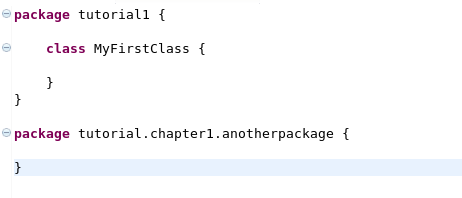
\includegraphics[scale=0.5]{images/tut1-001.png}

\noindent
You can observe the following:
\begin{itemize}
  \item Syntax highlighting. Keywords such as {\ttfamily package} or {\ttfamily class} are displayed in a different color,
  comparable to Java syntax highlighting.
  \item Source folding. You see small encircled minus signs at the left side. Click on them to collapse or expand the corresponding scope areas.
  \item Auto-completion.  If you type {\ttfamily packa} and then press ctrl-space, Eclipse will auto-complete the keyword {\ttfamily package}.
  In case of multiple possibilities, you will get a popup window with all expansions valid in the current context.
  \item Online syntax checking. Enter a class name which starts with a lower case letter.

\vspace{2mm}

\hspace{1cm}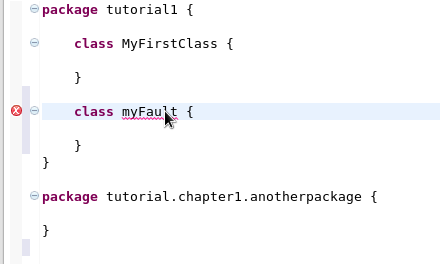
\includegraphics[scale=0.5]{images/tut1-002.png}

    \noindent
    If you move the mouse above the keyword underlined with the way red line, Eclipse will show a tooltip with the explanation
     ``Class names should start with upper case letters''.

\end{itemize}

Delete the class with the incorrect name. We want to add some fields to the class {\ttfamily MyFirstClass} now. As a type keyword, Bonaparte supports all
primitives and their boxed equivalents of Java (which, for the Java code generator, map exactly to their corresponding Java equivalent), plus the following additional types:

\begin{itemize}
  \item Character types:  {\ttfamily Ascii}, {\ttfamily Lowercase}, {\ttfamily Uppercase}, {\ttfamily Unicode}. In Java, all of them map to {\ttfamily String},
   but they have different plausibility checks in the deserializer. The {\ttfamily Ascii} type accepts the printable 7 bit ASCII characters
    (code points 0x20 to 0x7e), therefore you know characters in these fields can be represented in any encoding, and they
    occupy a single byte only in the UTF-8 encoding. They represent the most portable subset of characters. They have a special type, because they are often used as the allowed subset for
      alphanumeric IDs. {\ttfamily Lowercase} and {\ttfamily Uppercase} are subsets of {\ttfamily Ascii}, which allow the characters {\ttfamily 'a'..'z'},
      respectively {\ttfamily 'A'..'Z'} only. These types are useful for ISO codes such as ISO 4217 currency codes or ISO 3166
      country codes, or ISO 639 language codes.
      The {\ttfamily Unicode} finally allows all know character codes, including multi-byte codes such as Japanese Kanji. It
      allow the tab character as well.
      It has an option {\ttfamily allowControlChars}, which also allows the other control characters such as line feeds as part of the content.
  \item Numeric types: {\ttfamily Int}, {\ttfamily Number}, {\ttfamily Decimal}.  {\ttfamily Int} is no special type, just a synonym for {\ttfamily Integer},
      provided to ensure that a capitalized keyword for any primitive data type represents it's boxed equivalent, which in Java is unfortunately a bit inconsistent.
      {\ttfamily Number} is a subset of {\ttfamily BigInteger} which requires the specification of the maximum allowed number of
      digits (currently, up to 38 digits are supported). {\ttfamily Number(3)} for example allows the mantissas from 0 to 999.
      The {\ttfamily Decimal} type requires the specification of significant digits and fractional digits. It is mapped to a type which supports fixed point BCD arithmetic, suitable for
      financial calculations, where the use of {\ttfamily float} or {\ttfamily double} is a no-go due to potential rounding issues. The {\ttfamily Decimal} type
      maps to the Java type BigDecimal. {\ttfamily Decimal} allows up to 18 significant digits. The number of fractional digits cannot exceed the number of significant digits.

      A length can be provided also for the Java primitives and their boyed equivalents, if given, it determines the maximum
      number of accepted digits. {\ttfamily short(4)} for example allows the numbers 0 to 9999 (possible with a sign, unless
      the {\ttfamily unsigned} attribute has been given). You can provide even decimal digits, for example {\ttfamily
      short(4,2)}. Depending on the serialization format, the short with the value 314 will then be sent as either 3.14 (XML,
      CSV type formats) or 314 (Bonaportable and compact format).
  \item Temporal types: {\ttfamily Day}, {\ttfamily Time}, {\ttfamily Timestamp}, and {\ttfamily Instant}. The {\ttfamily Day}
  type represents a calendar date without time. In Java, it maps to the {\ttfamily LocalDate} class of the JodaTime library. The {\ttfamily Timestamp} type represents an instant (day plus time), which in Java maps
    to the {\ttfamily LocalDateTime} class of the JodaTime library. In serialized form, the timestamp is always in UTC time zone. For {\ttfamily Timestamp},
    you can specify a sub-second precision of 0 to 3 (0 meaning single second precision, 3 meaning millisecond precision).
    The {\ttfamily Instant} finally is there to support the JodaTime {\ttfamily Instant} class.
    As Java 8 includes JSR310, you can also configure the DSL to use Java 8 classes instead of the JodaTime classes, as all
    supported JodaTime classes have a Java 8 equivalent. There is an important difference concerning the serialized form,
    between {\ttfamily Timestamp} and {\ttfamily Instant}: {\ttfamily Instant} will be transmitted as 64 bit long integer,
    specifying the number of milliseconds since the epoch, while {\ttfamily Timestamp} is serializes as a decimal, with the
    integral part representing the date in YYYYMMDD format, and the fractional digits the time of day, in either hhmmss
    format, or in (milli)seconds of the day.
  \item Binary data: {\ttfamily Binary}, {\ttfamily Raw}: The {\ttfamily Binary} data type maps to a Java type supplied by Bonaparte itself, which is an
    equivalent to the Java {\ttfamily String} type: immutable, supporting subsets of contents without the need to perform deep copies of the underlying buffer etc.
    The {\ttfamily Raw} data type maps to the Java standard {\ttfamily byte []} type. Its use is discouraged and will cause warnings, because
    {\ttfamily byte []} is not immutable and has weird syntax concerning ordering of indexes, when itself part of an array.
    In the Bonaparte serialization format, the content of both types are represented in a nonstandard base64 encoding (nonstandard with respect to omission of
    newlines after every 60 characters, as required by the RFC. Those newlines would break the overall Bonaparte message format).
  \item Other types: {\ttfamily Uuid}, {\ttfamily Object}, {\ttfamily Enum} and {\ttfamily Xenum}. The
  {\ttfamily Uuid} type supports the universally unique identifiers (\url{http://en.wikipedia.org/wiki/Uuid}) and their standardized transmission format as a 36 byte hex string, formatted with dashes.
   The type maps to the Java UUID class. The {\ttfamily Object} holds a generic type defined in Bonaparte. A type (or subtype) of a specific class can be
    referenced by giving it's name in round parenthesis.
   The {\ttfamily Enum} references a special enumeration class, also defined in Bonaparte, which will be discussed later.
   {\ttfamily enum}s can be either regular (as in Java, identified by some integral ordinal), or alphanumeric ({\ttfamily
   Tokenizable}, where a string can be used to identify the instance). The latter one is preferred, because additional instances
   can be added in a portable way, and indenpendent of the order of reference. The {\ttfamily Xenum} references an extended
   enum, for which some kind of inheritance (allowing the addition of instances) is allowed. {\ttfamily Xenum}s always build on
   top of {\ttfamily Tokenaizable} {\ttfamily enum}s.
   \item Sets of enums and xenums are supported as well, these are comparable to the Java {\ttfamily EnumSet} class, but allow
   access to the underlying bitmap. For {\ttfamily enumset}s, all primitive integral types are supported for the bitmap. In
   addition, an {\ttfamily enumset} can be represented by the concatenated list of tokens, provided the tokens are all single
   characters. Such sets are always stored in ascending order of the token, such that the representation is deterministic, and
   it is possible to define simple regular expressions matching all enum sets which contain a specified subset of instances.
   \item External type adapters. Any Java Class can be used within Bonaparte, if a suitable type adapter is provided. Type
   adapters work similar to JAXB's {\ttfamily XmlAdapter}s. Bonaparte distinguishes {\ttfamily singleField} adapters, which map
   to a single directly supported Bonaparte type (i.e. one of the above), or arbitrary adapters, which map through some
   intermediate support class, described by a list of Bonaparte types (including previously defined adapters).

   An adapter can receive input from a separate previously defined field. This way a class using a number of money types for
   example can be serialized, transmitting the currency only once.
\end{itemize}

To extend the primitives vs. boxed types relationship, all these additional types can also be used in lowercase. In Java, they will still be implemented as
classes, but with the corresponding property that they don't accept null as a valid value when parsing input from the serialized forms.

\vspace{2mm}

Any integral type can be specified with a maximum number of digits, for example {\ttfamily Long(12)}. This is very useful when
building interfaces to languages or systems using fixed width formats, like COBOL or SAP (IDOC).

You can even specify the number of some (assumed) fractional digits, for example {\ttfamily Long(18,6)}. Some formats (CSV, XML)
will transmit the numbers as fractional numbers then, while the internal representation will be integral. This feature is
intended to support building interfaces for the fixed point arithmetic of the upcoming JSR-354 (money API).


\vspace{2mm}

As an exercise, try some types and save the file {\ttfamily .bon} file. The default configuration is that Eclipse automatically transforms the source into
Java code during the save process (which can be configured via the standard Eclipse project setting ``build automatically''). The generated code goes into
{\ttfamily src-gen} by default, but the recommendation is to change that to {\ttfamily src/generated}, to match Maven folder conventions.
This can be done per project or via global workspace settings, in the ``BonScript'' section.

\vspace{2mm}
\begin{center}
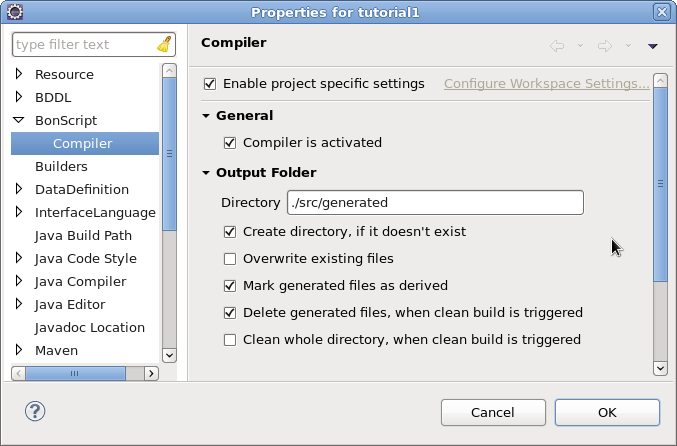
\includegraphics[scale=0.45]{images/tut1-003.png}
\end{center}

There are some more settings you can adjust in order to adapt the code generator to your needs:

\vspace{2mm}
\begin{center}
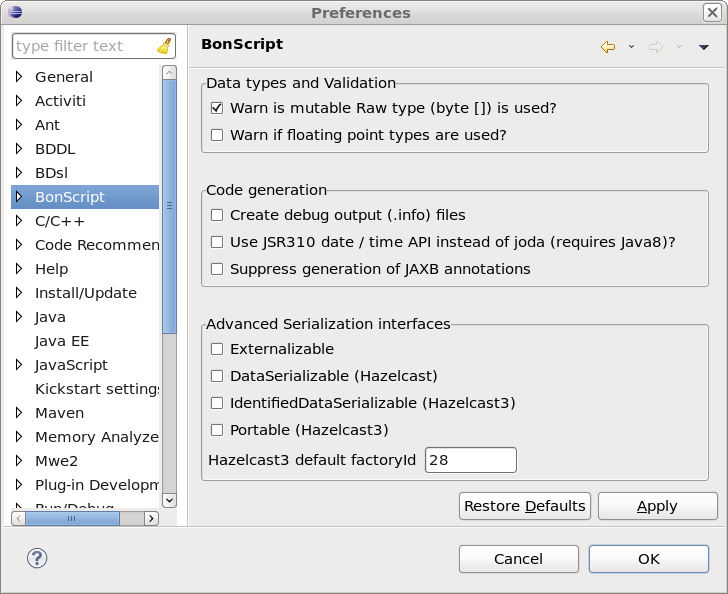
\includegraphics[scale=0.5]{images/tut1-prefs2.png}
\end{center}

Look into the generated code. It will have tons of unnecessary imports, but otherwise should be pretty much readable.
You will notice that the generated class implements two interfaces, {\ttfamily Externalizable} and {\ttfamily BonaPortableWithMetaData}.

\vspace{2mm}
\hspace{1cm}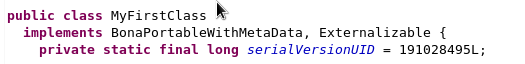
\includegraphics[scale=0.5]{images/tut1-004.png}

\noindent
The {\ttfamily Externalizable} interface indicates that there is a customization of way the object is serialized when initiated
via the standard Java serialization (namely {\ttfamily readExternal} and {\ttfamily writeExternal} are implemented) (and this behaviour can be disabled),
the other interface is the for the standard Bonaparte interface. Ignoring the metadata part, all Java classes generated by Bonaparte implement the interface
 {\ttfamily de.jpaw.bonaparte.code.BonaPortable}. This is the interface you should reference for fields which hold any object created by the Bonaparte grammar.


Apart from these, you see implementations of {\ttfamily hashCode} and {\ttfamily equals} (which behaves as expected, comparing the contents of
the instances), as well as getters and setters for the fields.

\section{Field visibility}
By default, fields in the generated classes have default visibility (can be accessed directly from other classes in the same package). This can be changed by
specifying a visibility directive exactly as in Java:

\vspace{2mm}
\hspace{1cm}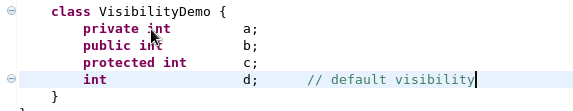
\includegraphics[scale=0.5]{images/tut1-006.png}

\noindent The generated code is as follows:

\vspace{2mm}
\hspace{1cm}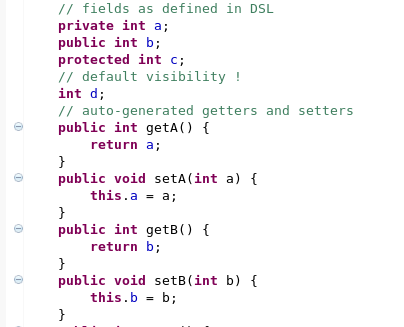
\includegraphics[scale=0.5]{images/tut1-008.png}

\noindent The getters and setters are always public.

\section{Class inheritance}
The availability of the {\ttfamily protected} keyword suggests that class inheritance is spported. In fact, you have exactly the same
possibilities as in Java: abstract and final classes, and single inheritance, using exactly the same syntax as in Java:


\vspace{2mm}
\hspace{1cm}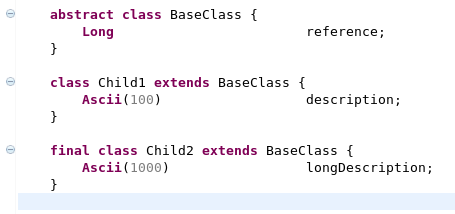
\includegraphics[scale=0.5]{images/tut1-007.png}


\section{Field specific parser directives}
Up to now, there's not a lot which would justify the overhead of a DSL.
We now want to provide directives to the parser which instruct it when to accept and when to reject data.

Any field you can prefix with the {\ttfamily required} keyword, which tells the parser to reject any record where no data for this field is specified.
This ensures, that in Java, you do not get {\ttfamily null} as the field value. (In other words, a {\ttfamily required
Ascii(10)} field would be equivalent to the notation {\ttfamily ascii(10)}.
The prior one offers better readability, and we will learn another use of the {\ttfamily required} keyword in a later chapter.)

For numeric fields, you can prefix them with the {\ttfamily unsigned} keyword. The parser will then reject negative values.

Alphanumeric fields allow the following directives:
\begin{itemize}
  \item {\ttfamily trim} instructs the parser to discard any leading or trailing space. Input data with field with the contents ``\ \ \ Some text\ \ \  '' would result in a String with the
  value ``Some text''. Any checks for maximum field length are performed after trimming spaces.
  \item {\ttfamily truncate} causes the parser to silently truncate data after the specified maximum field length has been reached.
   (The default behaviour is to reject data when field contents exceeds the specified length.)
   \item {\ttfamily regexp} {\it{some string}} causes the parser to validate the data against any regular expression. (This is only supported for
     {\ttfamily Ascii} fields or their upper/lowercase subtypes).
   \item Instead of just maximum field lenghts, you can also specify minimum number of character by giving a range as the field size.
    {\ttfamily Unicode(10..100) description} does require a description of at least 10 characters.
\end{itemize}

This screenshot shows a class where the directives explained above are used:

\vspace{2mm}

\hspace{1cm}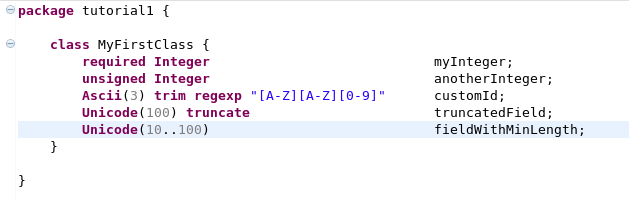
\includegraphics[scale=0.5]{images/tut1-005.png}

Numeric fields with fractional digits (type {\ttfamily Decimal} allow the following directives:
\begin{itemize}
  \item {\ttfamily round} instructs the parser round any input with more fractional digits to the number of fractional decimals
  specified. Gaussian rounding (also known as Banker's rounding / twopenny rounding / half-to-even
  \url{http://en.wikipedia.org/wiki/Rounding#Round_half_to_even}) is used for this. This is also the default IEEE 754 rounding
  mode. space.
  \item {\ttfamily failOnExtraDecimals} Opposite of {\ttfamily round}, tells the parser to throw an exception if input if more
  decimal digits is provided. Use this for financial data. This is also the default setting, but the directive is required if
  {\ttfamily round} has been specified as package or class default.
  \item {\ttfamily autoScale} instructs the parser return any parsed data scaled to exactly the specified number of decimals
  (useful in Java to compensate for the odditiy of the {\ttfamily BigDecimal} class, namely that 2.5 not equals 2.50.
  \item {\ttfamily noScale} Opposite of {\ttfamily autoScale}, tells the parser to return data as provided (i.e. in Java,
  the receiving application can determine the actual number of trailing zeroes sent, unless they exceed the maximum number, in
  which scaling is applied regardless. This is the default setting.
\end{itemize}

\section{Default settings}
Often, some settings apply to a whole class or package.
In Bonaparte, you can define field visibility and also some of the field specific parser directives at package and class level.

Suppose, you only deal with unsigned numeric data and also have one class where all parsed data should be stripped from leading and trailing space.
You also want all fields to be publicly accessible:

\vspace{2mm}

\hspace{1cm}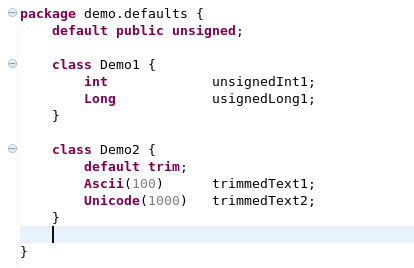
\includegraphics[scale=0.5]{images/tut1-009-defaults.png}

\noindent You can override every default directive at the deeper level, for example override package default per class or per field and override class defaults
at field level. For this purpose, for every directive, there is a corresponding negated directive.
The following default directives are supported:
\begin{itemize}
   \item {\ttfamily enum}, {\ttfamily noenum} (apply to all enum fields): Specifies whether new class instances should
   initialize enums with the token defined first.
  \item {\ttfamily public}, {\ttfamily private}, {\ttfamily protected}, {\ttfamily default} (applies to all fields): Specifies the visibility. The keyword
   {\ttfamily default} is required to restore default visibility when a different one has been set before.
   \item {\ttfamily signed}, {\ttfamily unsigned} (apply to all numeric fields): Specifies whether negative numbers are accepted or rejected.
   \item {\ttfamily required}, {\ttfamily optional} (apply to all fields which have an uppercase type): Specify whether an empty field is parsed as
    {\ttfamily null} or is rejected. Obviously you cannot specify {\ttfamily optional} for primitive types, and for consistency also not for other types which
    are the lowercase equivalent of the main type.
  \item {\ttfamily trim}, {\ttfamily notrim} (apply to {\ttfamily Unicode}, {\ttfamily Ascii}, {\ttfamily Lowercase}, {\ttfamily Uppercase} fields):
    Specify stripping of leading and trailing whitespace.
  \item {\ttfamily truncate}, {\ttfamily notruncate} (apply to the same types): Specify if encountering oversize input will cause silent truncation or throwing an exception.
  \item {\ttfamily round}, {\ttfamily failOnExtraDecimas} (apply to {\ttfamily Decimal} fields): specifies whether too many
  non-zero fractional digits are rounded or an exception is thrown.
  \item {\ttfamily autoScale}, {\ttfamily noScale} (apply to {\ttfamily Decimal} fields): specifies
  whether returned {\ttfamily BigDecimal} instances in Java are all scaled to the specified number of decimals.
  \item {\ttfamily allowControlChars}, {\ttfamily noControlChars} (apply to {\ttfamily Unicode} fields): specifies whether special characters such as line feeds are accepted.
    The Bonaparte format will escape them properly such that they do not break the format, but if you export data to regular CSV files as well, you might want to
    forbid such characters.
  \item {\ttfamily usePrimitives}, {\ttfamily useBoxed} (applies to types which have Java primitive type equivalents): Instructs the generator to use the primitive types
    or to use only boxed types.
\end{itemize}
The directives must appear in the order given above. Defaults do not extend to additional fields in inherited classes.

\section{Type definitions}
An important feature missing in the Java language is the ability to assign a logical name to a type (this is even worse because Java also does not support a preprocessor,
which could be used as a fallback). The ``Java way'' to define a class for such purpose is loaded with the burden of additional memory / performance overhead
and also requires its own source file. The Bonaparte DSL fills this gap, allowing a very lean possibility to define user types.

Assume you design a financial application and need currency codes frequently. The use of {\ttfamily Uppercase(3)} just isn't self-documenting, because it could
also mean a 3-character country code.
In Bonaparte, you can define and later use a type definition as follows:

\vspace{2mm}

\hspace{1cm}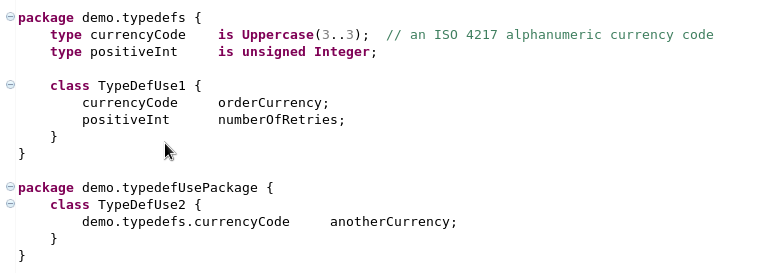
\includegraphics[scale=0.5]{images/tut1-010-typedefs.png}

\noindent
Type definitions must appear in packages before any classes are defined. As shown in the example, you can also use them in other packages,
specifying their fully qualified name. This is not very convenient, a simpler way is shown in the next section.

A very important aspect of type definitions is, that they bind package / class defaults from where they are defined, and not where they are used.
This decision has been made in order to ensure that a type has the same properties everywhere.


\section{Combining multiple source files}
As projects get bigger, it is no longer convenient to have all definitions inside a single file.
The Bonaparte DSL supports multiple source files, and definitions made in one file can be imported and used in another file.


The {\ttfamily import } statement specifies, which data should be imported. You can import specific elements or use wildcard imports as shown.

\vspace{2mm}

\hspace{1cm}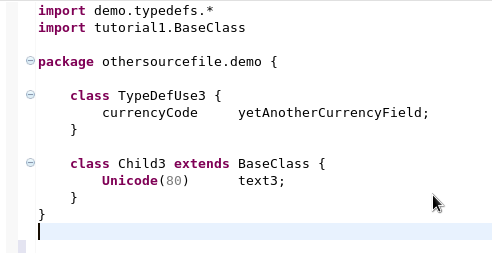
\includegraphics[scale=0.5]{images/tut1-011-imports.png}

\noindent Imports include the imported data into the current namespace, therefore se of the fully qualified name is no longer required.
Bonaparte supports imports only at the beginning of a source file, before any package is defined. Please note that the logical package of
the imported data must be specified, do not mix it up with C's {\ttfamily \#include}, which references a file location.

\section{Javadoc}
Bonaparte will copy Javadoc comments created just ahead of a class definition to the generated class source. In addition, Javadoc style
multiple comments just ahead of a package definition will by transferred to a special {\ttfamily package-info.java} file.
If you use the same package name in multiple source files, you are responsible to take care that no conflicts concerning
class names or package Javadoc occurs. (If there are conflicts, the one generated last would overwrite prior definitions.)

Regular single-line comments which appear behind a field definition will be copied to the generated Java source file.
(Plan is to convert it to field level Javadoc, at the moment the required value converter has not yet been implemented.)

\newpage

\section{Enums}
As briefly mentioned before, enumeration data types are supported as well.

Their key purpose here is to offer self-documenting values for use in applications, and mapping these to very short tokens
for transmission in serialized forms (usually one or two characters).
Enum definitions have to appear below typedefs, but above class defintions.
The syntax is very close to Java syntax. Enum references must start with the {\ttfamily enum} or {\ttfamily Enum} keyword
 (for required / nullable enumerations) and the enum reference should always start with an uppercase letter.
All enum classes generated by the Bonaparte DSL will either implement {\ttfamily BonaNonTokenizableEnum} or {\ttfamily BonaTokenizableEnum}
(both interfaces extend the common interface {\ttfamily BonaEnum}).

\vspace{2mm}

\hspace{1cm}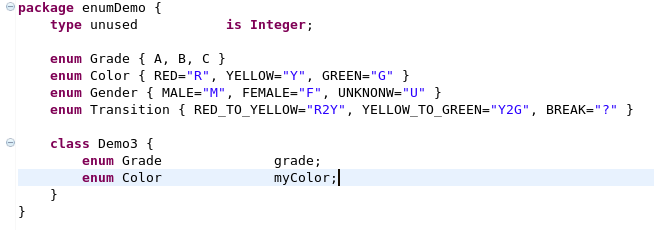
\includegraphics[scale=0.5]{images/tut1-013-enum.png}

\noindent The mappings of tokens to string equivalents must either be provided for all values or for none. If the mapping is provided, the
mapped strings will be used in the serialized form.


\section{Extensible Enums}
Extensible enumeration data types allow adding instances throug inheritance.

As Java does not allow this for native enums, an {\ttfamily xenum} will create a wrapper class, which is a regular Java class,
and which holds a reference to the underlying enum. {\ttfamily xenum} classes only support {\ttfamily enum}s with alphanumeric
tokens. At runtime, all inheriting classes must be loaded before the functionality works as expected.

\vspace{2mm}

\hspace{1cm}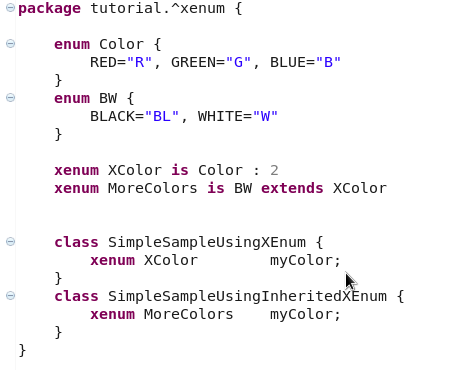
\includegraphics[scale=0.5]{images/tut1-xenum.png}

The purpose of the {\ttfamily :2} specifier in the definition of the base xenum {\ttfamily XColor} is to provide the maximum
token length for subclasses. If not specified, the maximum length of all tokens of the base enum will be used.


\section{Class references}
A very important aspect is the ability to reference other classes. This is done by referencing the class in in round parenthesis.
Such a reference can either be valid for exactly the referenced class (no subclasses), or for any class in the inheritance hierarchy below or equal to
 the referenced class. In the latter case, append dots to the type reference.

\vspace{2mm}

\hspace{1cm}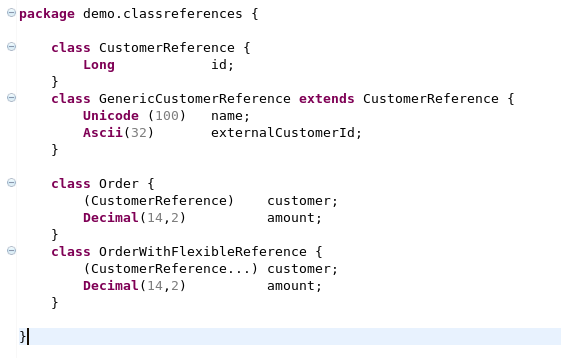
\includegraphics[scale=0.5]{images/tut1-014-ref.png}

\noindent In this example, the {\ttfamily Order} class can only have a customer reference given by artificial key, while the {\ttfamily OrderWithFlexibleReference}
would accept a {\ttfamily CustomerReference} or {\ttfamily GenericCustomerReference} (or any other subclass) and would need to be able to resolve all these
references. (Again, this check is only implemented when parsing serialized messages. As Java does not support such functionality, nothing prevents you
from assigned an instance of {\ttfamily GenericCustomerReference}  to the {\ttfamily Order.customer} field directly in Java.



\section{Arrays, Lists, Sets and Maps}
Often, fields do not occur a single time only. Bonaparte supports arrays, lists, sets and maps. All except maps are
serialized to the same format, therefore switching between both alternatives does not break message compatibility.
Use which ever is better suitable for your application.
Both forms can optionally specify a maximum number of entries.
The syntax for arrays is similar to Java, the list / set / map syntax differs from Java (for sake of grammar simplicity).

\vspace{2mm}

\hspace{1cm}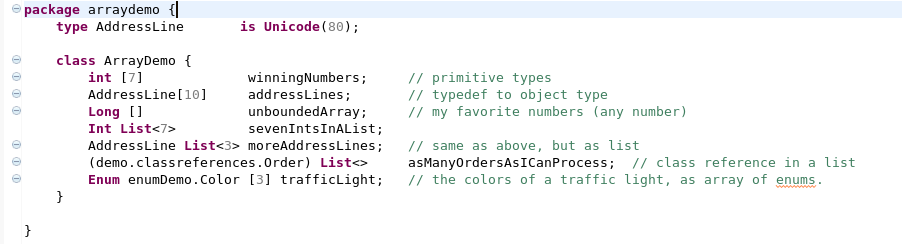
\includegraphics[scale=0.5]{images/tut1-015-arrays.png}

For collection types, you can specify at two levels, if {\ttfamily null}s are allowed: for the collection itself, and for the
collection elements.  The recommendation is to set collection elements always to {\ttfamily required}. There are some
implementations, which also require that, for example most classes of the Google {\ttfamily guava} library (see
\url{http://code.google.com/p/guava-libraries/wiki/LivingWithNullHostileCollections}).

\vspace{2mm}

\hspace{1cm}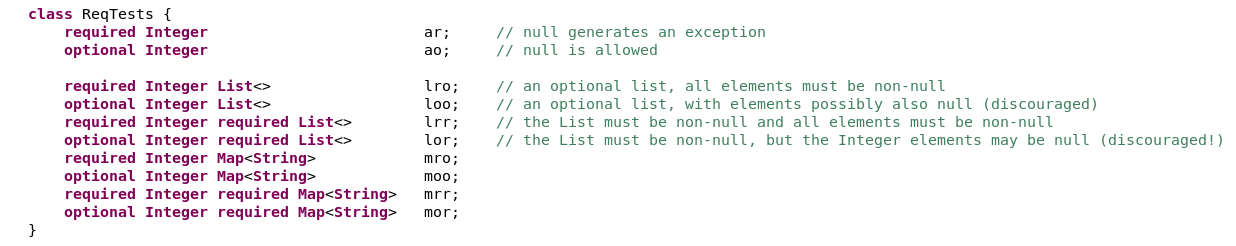
\includegraphics[scale=0.5]{images/tut1-016-collections.png}


\section{Sets of enums}
For eenumsets, it is important to know that their iterator will always provide the instances in a defined ordering: for
sets using a bitmap for storage, it is by ascending ordinal, for concatenated token storage in strings, it is by ascending
token.

\vspace{2mm}

\hspace{1cm}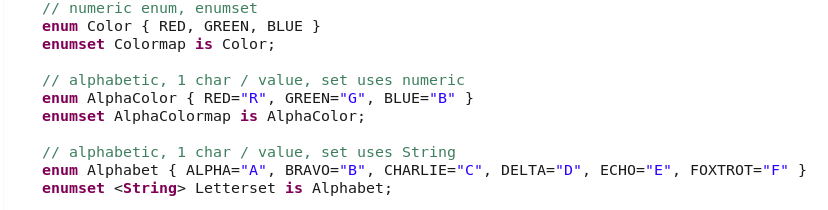
\includegraphics[scale=0.5]{images/tut1-enumsets1.png}

Their use is accordingly:

\vspace{2mm}

\hspace{1cm}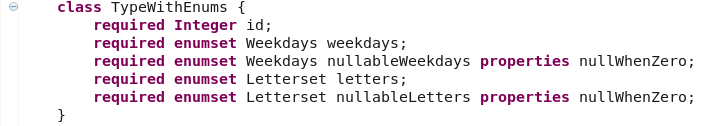
\includegraphics[scale=0.5]{images/tut1-enumsets2.png}

Please note the {\ttfamily properties nullWhenZero} addition, this does not have any effect in the main Bonaparte DSL, but is
evaluated by the Bonaparte JPA DSL: The effect is that if such a class is stored in a database, empty sets will be stored as
{\ttfamily null} in case of 0, resp. {\ttfamily ""}, optimizing index size.


\section{Generics}
All generic references in Bonaparte specify classes defined in Bonaparte, i.e. they map to the Java representation of {\ttfamily
? extends BonaPortable}. It is not possible to use generics to reference boxed primitives.

\section{Adapters}
The following code fragment allows storing an instance of {\ttfamily java.lang.Class} inside a Bonaportable:

\vspace{2mm}

\hspace{1cm}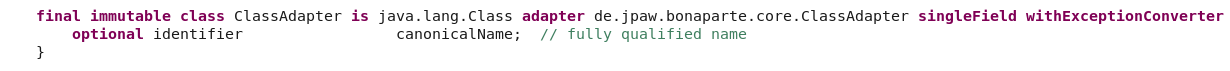
\includegraphics[scale=0.5]{images/tut1-adapter1.png}

The adapter is defined as follows:

\vspace{2mm}

\hspace{1cm}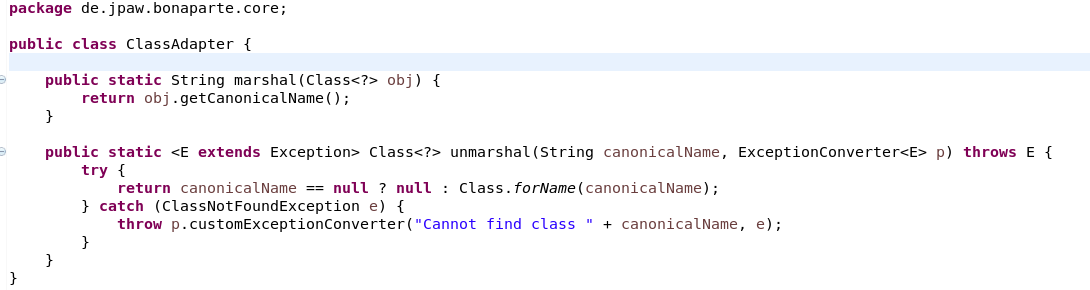
\includegraphics[scale=0.5]{images/tut1-adapter2.png}

An adapter consists of a {\ttfamily marshal} and an {\ttfamily unmarshal} method. The unmarshal method is always static, the
marshal method is an instance method, of the adapter is defined as part of the external class itself.
The marshal method is invoked after null checks have been performed, this allows to return primitive types, avoiding
unnecessary boxing / unboxing during serialization.

For the unmarshal, this is always responsibility of the adapter, because the return type is an object anyway.
The unmarshaller can receive an extra exception converter parameter; use this if the conversion can throw exceptions for invalid
input data. This allows to enrich the response with field and class name information and sometimes save you from digging
through stack traces.

The unmarshaller can also receive extra parameters. A more complex example of an adapter without extra parameter

\vspace{2mm}

\hspace{1cm}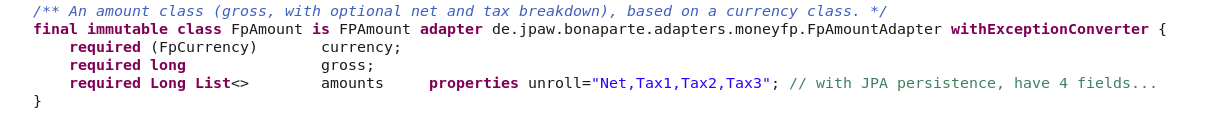
\includegraphics[scale=0.5]{images/tut1-adapter3.png}

looks like this with the extra parameter:

\vspace{2mm}

\hspace{1cm}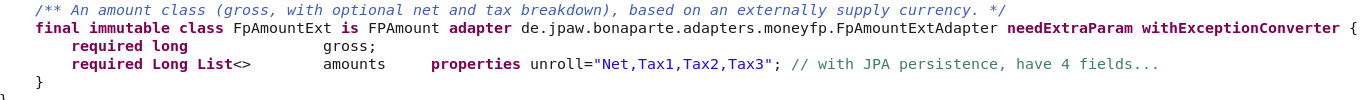
\includegraphics[scale=0.5]{images/tut1-adapter4.png}

Here, the first component has been omitted and is taken from another field of the class, which one is defined when the adapter
is used:

\vspace{2mm}

\hspace{1cm}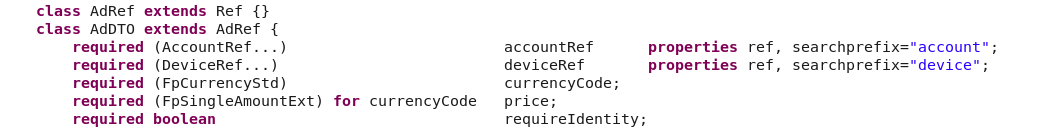
\includegraphics[scale=0.5]{images/tut1-adapter5.png}

In the example, the {\ttfamily currencyCode} field (which by coincidence is itself mapped by an adapter here) is used to provide
the missing information.

You can find more examples of adapters on the projects {\ttfamily bonaparte-adapters-}*.


\section{Special directives}
The following directives can be specified at package or class level, in the given order.
\subsection{JAXB directives}
Bonaparte can emit JAXB directives (in a very limited way), namely specifying the access type through directive {\ttfamily XML}, followed
by either {\ttfamily noXML}, {\ttfamily NONE}, {\ttfamily FIELD}, or {\ttfamily PROPERTY}. This causes the code generator to generate
appropriate JAXB annotations, and also to create a file {\ttfamily jaxb.index} at package level.


\subsection{Skipping the {\ttfamily Externalizable} interface}
If you do not want that Java's default serialization implementation is modified, specify {\ttfamily noExt}. (Specify {\ttfamily Ext} to
override a default done at package level.)

\subsection{JSR303 Bean Validation}
If you want to create JSR303 style annotations, specify {\ttfamily BeanVal}. (Specify {\ttfamily noBeanVal} to
override a default done at package level.)

\vspace{2mm}

\hspace{1cm}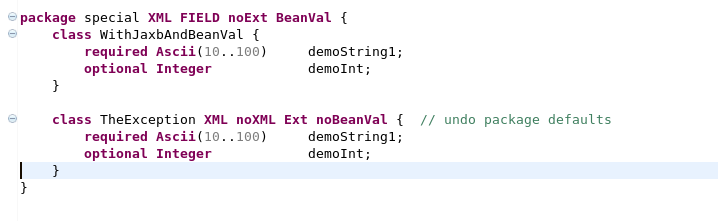
\includegraphics[scale=0.5]{images/tut1-012-special.png}

\noindent The generated code contains the following:

\vspace{2mm}

\hspace{1cm}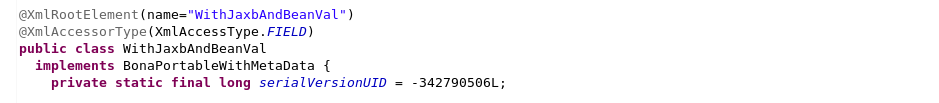
\includegraphics[scale=0.5]{images/tut1-012-special-1.png}

\ldots

\vspace{2mm}

\hspace{1cm}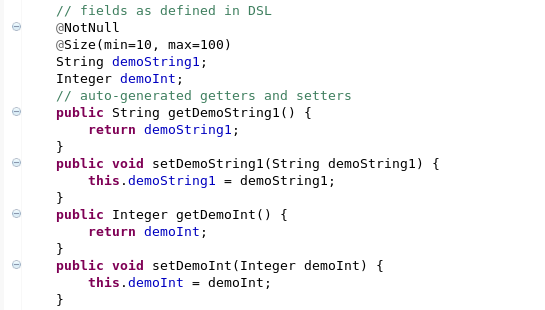
\includegraphics[scale=0.5]{images/tut1-012-special-2.png}

\end{document}
